\documentclass{article}
\usepackage[utf8]{inputenc}
\usepackage{csquotes}
\usepackage{natbib}
\usepackage{graphicx}
\usepackage{float} 
\usepackage{epsfig}
\usepackage{siunitx}
\begin{document}
\begin{titlepage}
	\begin{center}
		\Huge\textbf{EE-568 }\\
		\vspace{0.5cm}
		\Huge\textbf{HW-1}\\
		\vspace{0.5cm}
		\Huge\textbf{Torque in a Variable Reluctance Machine}\\
		\vspace{0.5cm}
		
\includegraphics[scale=1]{E:/Github/EE568/HW1/Rapor/Figurler/odtulogo}\\
		
		
		\Large\textbf{Prepared by:}Hakan POLAT\\
		
		\Large\textbf{Submitted to:} Dr. Ozan KEYSAN\\
		\vspace{0.5cm}
		\Large\textbf{Electrical and Electronics Engineering Department}\\
		
		\large\textbf{ANKARA	}\\
		\large\textbf{05.03.2020}\\
		
		
		
	\end{center}
	
	

\end{titlepage}

\newpage
\section{Introduction}
In this report a variable reluctance machine is investigated both analytically and numerically. In the first part, the system parameters will be delivered. In the next part, an analytic derivation for the reluctance and inductance will be made for the machine under investigation. The torque produced under DC excitation will be derived and presented. Then additional methods for improving the analitic approach will be discussed.\\
In the next part, results for 2D finite element model of the machine will be presented. The analysis is done in ANSYS Maxwell environment. The core material is selected as laminated steel and the permeability is taken as linear. The flux densities for degrees 0,45 and 90 are plotted. The inductance, stored energy and torque is calculated using finite element analysis. The results are then compared to the analytical results and the differences are discussed. \\
In the final part, a non-linear core material is selected. The effect of core saturation is observed. The analysis performed in previous section is repeated. Again the analysis results are compared to the analytical model and the linear core material cases and discussed.

\section{System Parameters and Dimensions}
The variable reluctance machine under investigation is presented in Fig. \ref{fig:system}. The machine constist of three parts. The coil windings are used to generated flux. The core is used to direct the flux and torque generated on the rotational section. The coils are wound within 30~mmx10~mm rectangle, each airgap clearance is 0.5~mm, depth of the core is 20~mm, number of turns is 250 and the excitation current is 3A~DC.
\begin{figure}[h!]
	\centering
	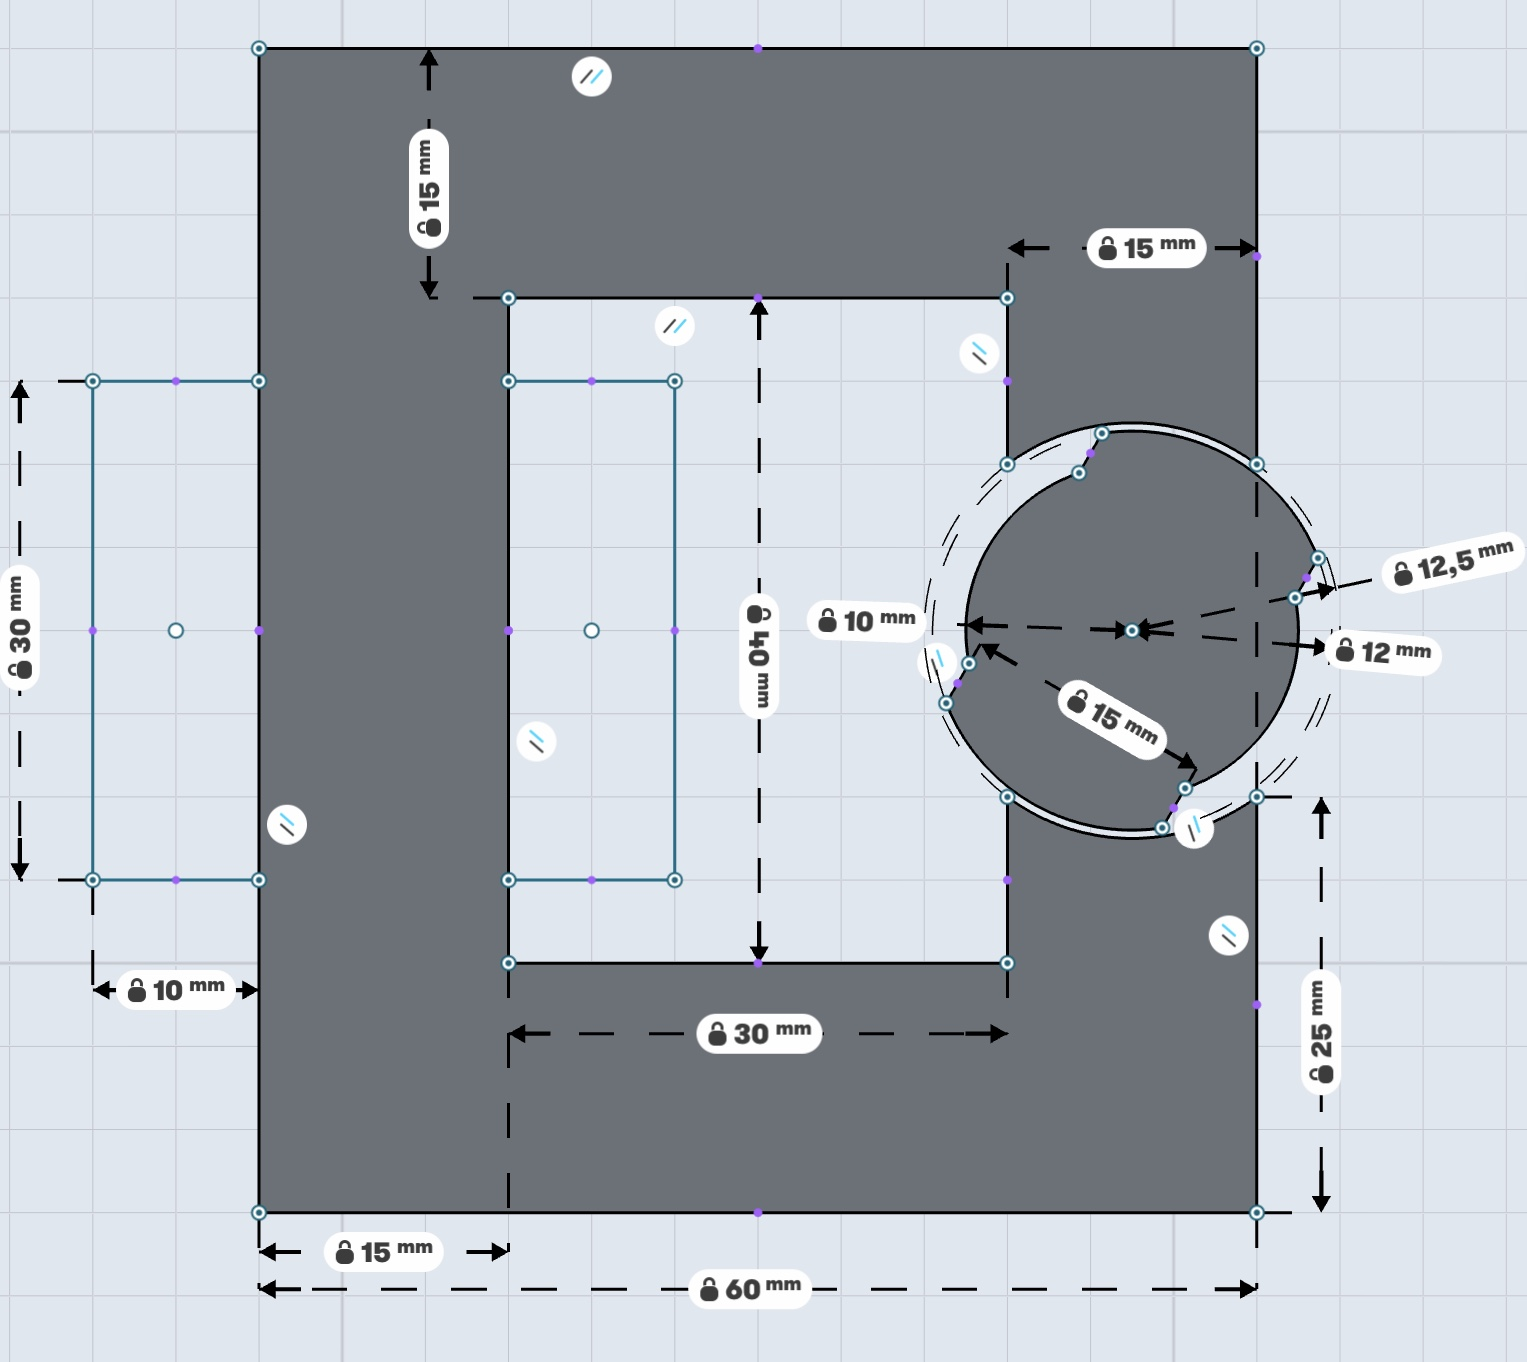
\includegraphics[width=0.5\linewidth]{Figurler/system.jpeg}
	\caption{2D CAD drawing of the variable reluctance machine under investigation.}
	\label{fig:system}
\end{figure}
\section{Analitical Modelling}
In the first subsection analytical modelling of the reluctance and inductance of the system will be made. Then the torque production of the machine will be derived and plotted.


\subsection{Reluctance and Inductance Modeling}
In order to derive an analitical formula for the reluctance and inductance some assumptions are made:
\begin{itemize}
	\item The core is infinitely permeable $\mu_{r}=\infty$,
	\item There is no leakage flux,
	\item The 0 degrees is set as in Fig. \ref{fig:initial}.
	\item The system is linear and hence there is no saturation.
\end{itemize}

\begin{figure}[H]
	\centering
	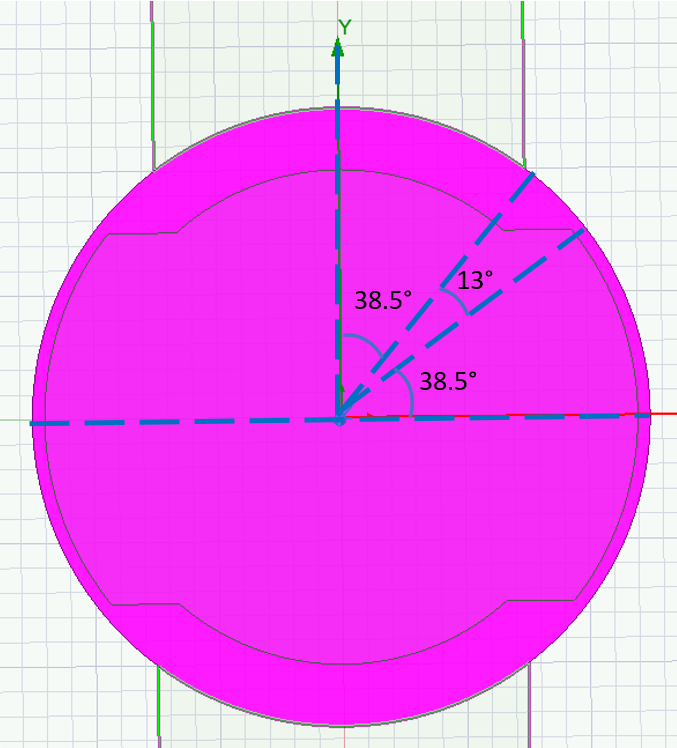
\includegraphics[width=0.7\linewidth]{E:/Github/EE568/HW1/Rapor/Figurler/initial}
	\caption{Initial rotor position set as $\theta=0 $}degrees
	\label{fig:initial}
\end{figure}
Since the system is assumed to be linear and infinitely permable the reluctance of the machine can be calculated as in (\ref{reluctanceformula}). \enquote{g} is the airgap and equal to 0.5~mm when rotor and the core is fully aligned and maximum 2.5~mm. \enquote{A} is the area between the rotor and the core. Calculation of \enquote{A} is given in (\ref{areaformula}). 
\begin{equation}
R=\frac{2g}{\mu_{0}A}
\label{reluctanceformula}
\end{equation}
\begin{equation}
A=20\frac{\ang{77}2\pi12.5 }{\ang{360}}=335~mm^2
\label{areaformula}
\end{equation}
Then the maximum and minimum reluctance of the machine can be calculated as in(\ref{reluctancecalculation}).
\begin{equation}
\begin{array}{l}
R_{min}=\frac{2g_{max}}{\mu_{0}A}=2.37\times 10^6 \frac{1}{H}\\  
R_{max}=\frac{2g_{min}}{\mu_{0}A}=11.87\times 10^6 \frac{1}{H}
\end{array}
\label{reluctancecalculation}
\end{equation}
At this point it is clear that $R_{min}$ point is achieved when there is a $\ang{90}$ of rotation and $R_{max}$ is achieved when rotation angle \enquote{$\theta$} is 
\ang{-13}$\leq$$\theta$$\leq$\ang{13} and \ang{167}$\leq$$\theta$$\leq$\ang{193}. The piecewise function of reluctance is presented in Table \ref{reluctancetable}.

	\begin{table}[h!]
		\centering
		\caption{Piecewice Function of Reluctance}
		\label{reluctancetable}
		\begin{tabular}{ll}
			\hline
			\ang{0}$\leq$$\theta$$\leq$\ang{13}	& $R=R_{max}$ \\ \hline
			\ang{13}$\leq$$\theta$$\leq$\ang{90}	&  Linear decrease from $R_{max}$ to $R_{min}$ \\ \hline
			\ang{90}$\leq$$\theta$$\leq$\ang{167}	& Linear increase from $R_{min}$ to $R_{max}$\\ \hline
			\ang{167}$\leq$$\theta$$\leq$\ang{180}	& $R=R_{max}$ \\ \hline
		\end{tabular}	
	\end{table}
Ampere law can be stated as in (\ref{amperelaw}) and inductance \enquote{L} can be calculated as in (\ref{inductanceformula}).
\begin{equation}
	NI=\Phi R 
	\label{amperelaw}
\end{equation}
\begin{equation}
L=\frac{\lambda}{I}=A\frac{\Phi}{I}=\frac{N^2}{R}
\label{inductanceformula}
\end{equation}
This equation is valid since $W_{stored}=W^{'}_{stored}$. It was our initial assumption that the system was linear. The maximum inductance($L_{max}$) occurs when there is minimum reluctance and minimum inductance $L_{min}$ occurs when there is maximum reluctance. The inductance of the system can be calculated as in (\ref{inductancecalculation}).

\begin{equation}
\begin{array}{l}
L_{min}=\frac{N^2}{R_{max}}=5.2 mH\\  

L_{max}=\frac{N^2}{R_{min}}=26.5 mH\\  
\end{array}
\label{inductancecalculation}
\end{equation}
Similarly a piecewise function of total inductance is presented in (\ref{inductancetable}).
	\begin{table}[h!]
	\centering
	\caption{Piecewice Function of Total Inductance}
	\label{inductancetable}
	\begin{tabular}{ll}

		\hline
		\ang{0}$\leq$$\theta$$\leq$\ang{13}	& $L=L_{min}$ \\ \hline
		\ang{13}$\leq$$\theta$$\leq$\ang{90}	& Linear increase from $L_{min}$ to $L_{max}$ \\ \hline
		\ang{90}$\leq$$\theta$$\leq$\ang{167}	& Linear decrease from $L_{max}$ to $L_{min}$ \\ \hline
		\ang{167}$\leq$$\theta$$\leq$\ang{180}	& $L=L_{min}$ \\ \hline
	\end{tabular}	
\end{table}
It is important to state that both inductance and reluctance functions are periodic. In Fig. \ref{fig:reluctanceanalitic} and Fig. \ref{fig:inductanceanalitic} a single period of reluctance and inductance are presented respectively.
\begin{figure}[H]
	\centering
	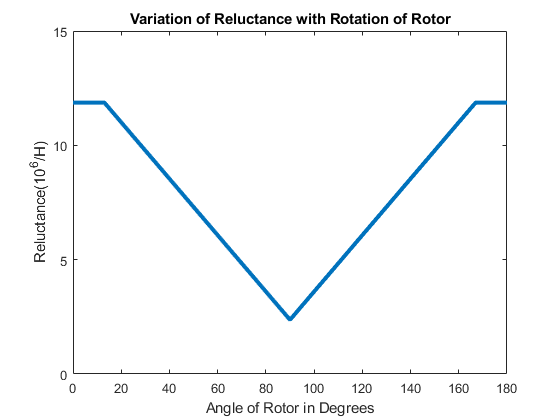
\includegraphics[width=0.7\linewidth]{E:/Github/EE568/HW1/Rapor/Figurler/reluctance}
	\caption{Variation of Reluctance with Rotation of Rotor}
	\label{fig:reluctanceanalitic}
\end{figure}
\begin{figure}[H]
	\centering
	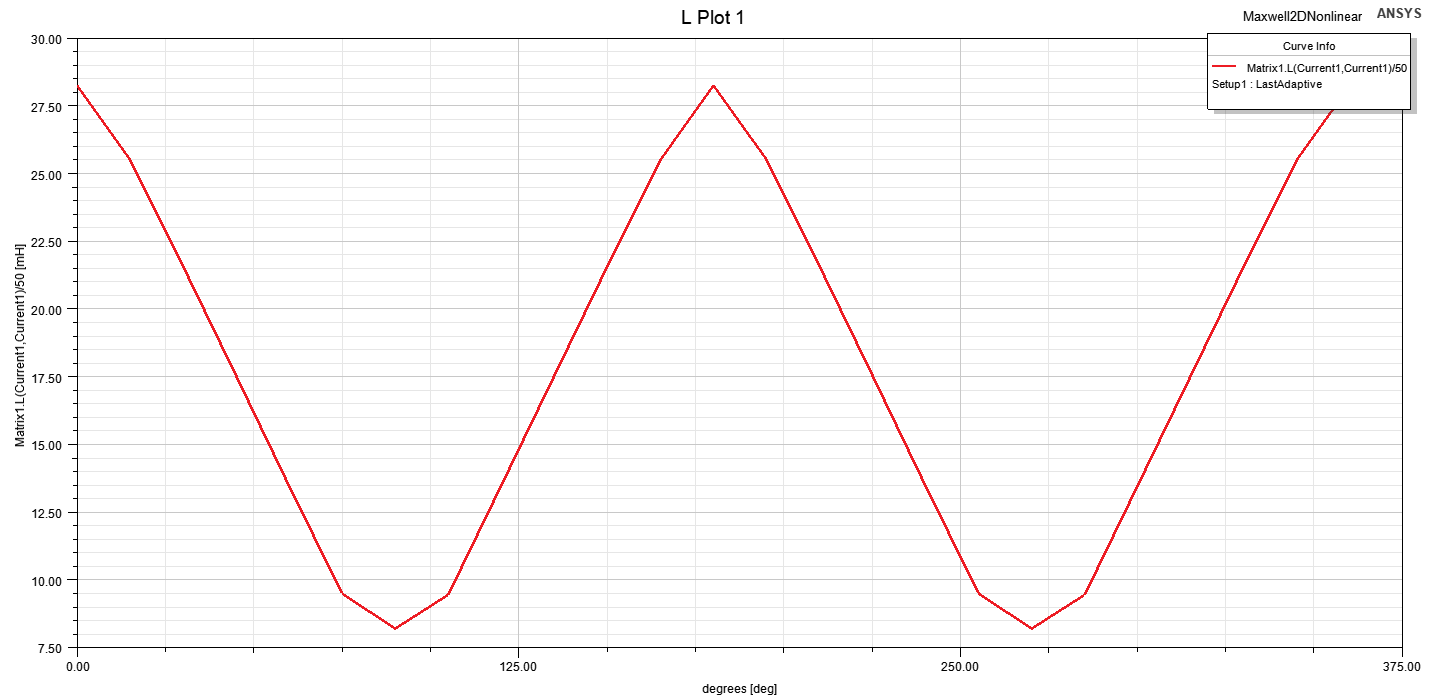
\includegraphics[width=0.7\linewidth]{E:/Github/EE568/HW1/Rapor/Figurler/inductance}
	\caption{Variation of Inductance with Rotation of Rotor}
	\label{fig:inductanceanalitic}
\end{figure}

\subsection{Torque Generation}
Since the system is linear $W_{stored}=W^{'}_{stored}=0.5LI^2$. Torque generation can be stated as in (\ref{torqueformula}).

\begin{equation}
T=-\frac{\delta W_{stored}}{\delta\theta}=\frac{\delta W^{'}_{stored}}{\delta\theta}=\frac{\delta(0.5LI^2)}{\delta\theta}=\frac{1}{2}I^2\frac{\delta L}{\delta\theta}=\frac{1}{2}I^2\frac{\Delta L}{\Delta\theta}
\label{torqueformula}
\end{equation}
Hence the piecewise torque generation can be written as in Table \ref{torquetable}. Here it is important to note that all degrees are converted to radians during calculations. Since \enquote{L} increases or decreases linearly the torque generation is constant. The generated torque is presented in Fig. \ref{fig:torqueanalitic}.
	\begin{table}[h!]
	\centering
	\caption{Piecewice Function of Torque Generation}
	\label{torquetable}
	\begin{tabular}{ll}		
		\hline
		\ang{0}$\leq$$\theta$$\leq$\ang{13}	& $T=0 Nm$ \\ \hline
		\ang{13}$\leq$$\theta$$\leq$\ang{90}	& $T=71 Nm$ \\ \hline
		\ang{90}$\leq$$\theta$$\leq$\ang{167}	& $T=-71 Nm$ \\ \hline
		\ang{167}$\leq$$\theta$$\leq$\ang{180}	& $T=0 Nm$ \\ \hline
	\end{tabular}	
\end{table}
\begin{figure}[H]
	\centering
	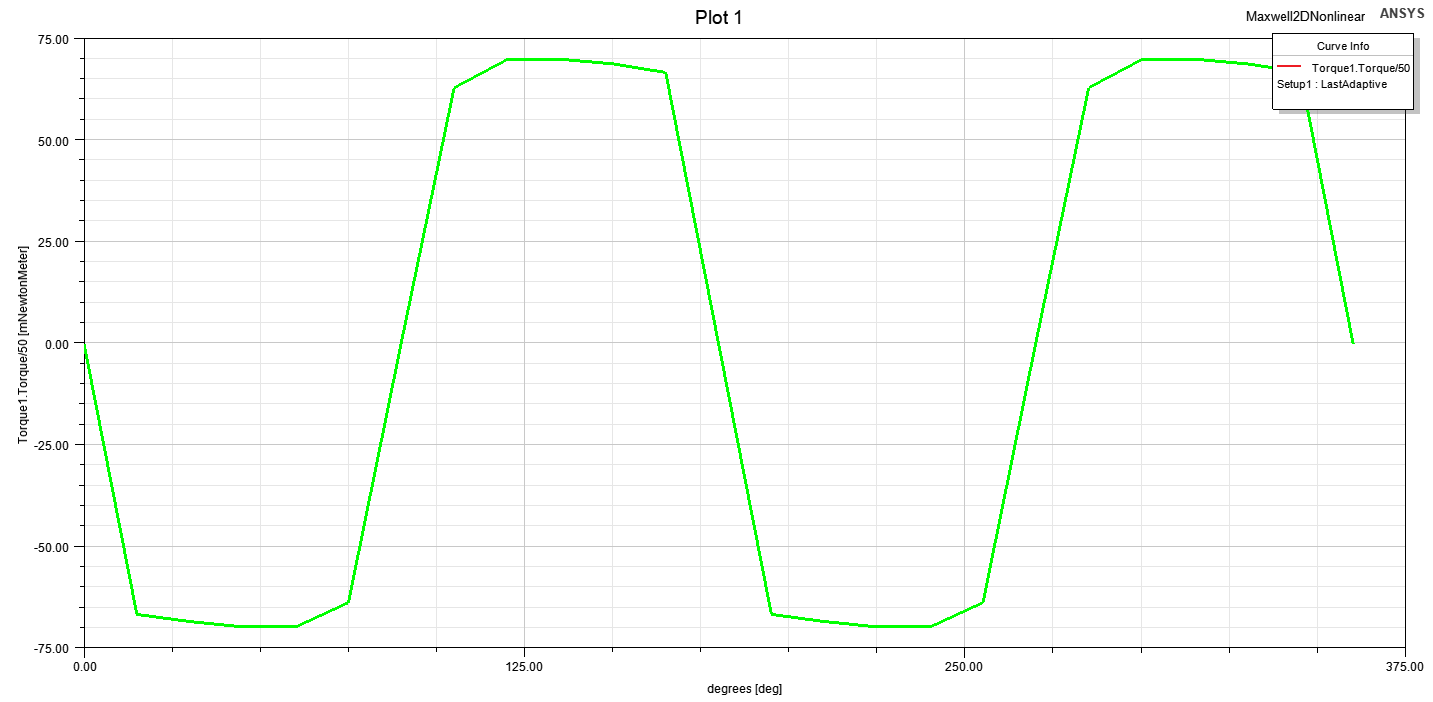
\includegraphics[width=0.7\linewidth]{E:/Github/EE568/HW1/Rapor/Figurler/torque}
	\caption{Variation of Torque with Rotation of Rotor}
	\label{fig:torqueanalitic}
\end{figure}

\subsection{Improvements}
The initial assumptions can be modified in order to achieve a better analitic approximation. The first change can be made to core permeability. In reluctance machines laminated steel is often the chosen material for its low cost and low core loss due to reduction of eddy losses. Iron has a relative permeability around 4000. This changes the total reluctance and hence changes the inductance and torque. A second approximation is on the flux path. Similar to current passing from minimum resistance, flux also tends to pass from loops with minimum reluctance. Hence normally the flux path is not distributed homogenously in the core but tends to concentrate close to the inner surface of the core material. 

\section{FEA Modelling(2D- Linear Materials)}
\section{FEA Modelling(2D- Non-Linear Materials)}
\section{Conclusion}

asdadasdas

\end{document}
